\section{Rund um den Kreis}
Autor: Marc Mittner

\noindent "Uberarbeitung: Christian Rutsch

\subsection{Definition}
Ein Kreis beschreibt die Menge aller Punkte, die von einem gegebenen Mittelpunkt aus den gleichen Abstand haben -- oder als mathematisch saubere Definition:
\[ K = \lbrace X \in E ,\  |\overline {MX}| = r \rbrace \]
(Erl"auterung: Der Kreis $K$ ist eine Menge, die alle Punkte $X$ einer Ebene $E$ enth"alt, f"ur die gilt, dass die L"ange der Strecke $\overline{MX}$ gerade den Radius $r$ ergibt.)

\subsection{Mathematische Beschreibung}
F"ur die mathematische Beschreibung eines Kreises gibt es verschiedene M"oglichkeiten. Hier soll nur die Darstellung mit kartesischen Koordinaten behandelt werden.

\subsection{Koordinatengleichung}
Die Koordinatengleichung eines Kreises im kartesischen Koordinatensystem lautet:
\[ (x - x_M)^2 + (y - y_M)^2 = r^2 \]
Der Mittelpunkt des Kreises ist dabei $M = (x_M , y_M)$, der Radius des Kreises ist $r$.
Durch den Satz des Pythagoras wird klar, wie diese Beziehung zustande kommt:

\begin{center}
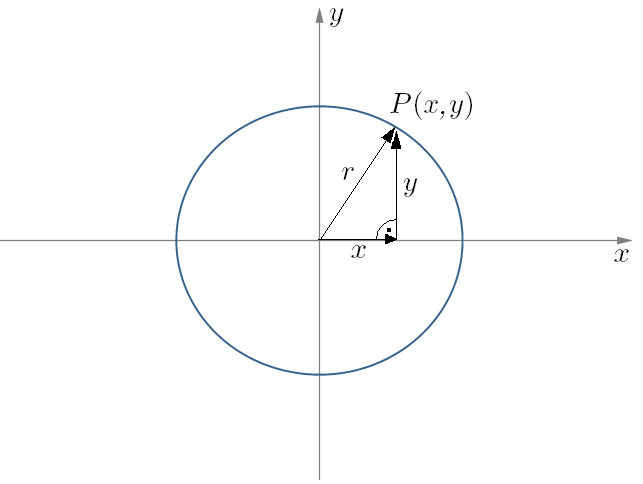
\includegraphics[scale=0.25]{img/kreis/kreis.png}
\end{center}

\noindent $x,\ y$ und $r$ bilden ein rechtwinkliges Dreieck. Also folgt aus dem Satz von Pythagoras (mit dem Mittelpunkt $M = \left({}^0_0\right)$):
\[ x^2 + y^2 = r^2 \]

\noindent Der Mittelpunkt des Kreises muss jedoch nicht zwingend der Ursprung des Koordinatensystems sein, sodass bei einer Verschiebung des Kreises in x- bzw. y-Richtung die folgende  Koordinatengleichung ensteht:
\[ (x - x_M)^2 + (y - y_M)^2 = r^2 \]

\noindent Ein wichtiger Begriff (grade f"ur die komplexen Zahlen (Kapitel~\ref{chap:complex}) sowie die Sinus- und Cosinusfunktionen (Abschnitt~\ref{sec:trigonometrie})) ist der Einheitskreis. Der Einheitskreis ist ein normaler Kreis um den Ursprung mit dem Radius $r=1$:
\[ x^2 + y^2 = 1 \]

\subsection{Funktionsgleichung}
Durch Umformen der Koordinatengleichung erh"alt man zwei Funktionsgleichungen zur Beschreibung des Kreises. Zum einen f"ur den oberen Teilbogen:
\[ y = y_M + \sqrt{ r^2 - (x - x_M)^2} \]
und f"ur den unteren Teilbogen:
\[ y = y_M - \sqrt{ r^2 - (x - x_M)^2} \]

\subsection{Beispiele}
\begin{enumerate}
    \item Der Einheitskreis mit Radius $r = 1$ um den Ursprung $M = (0 , 0)$:

\begin{center}
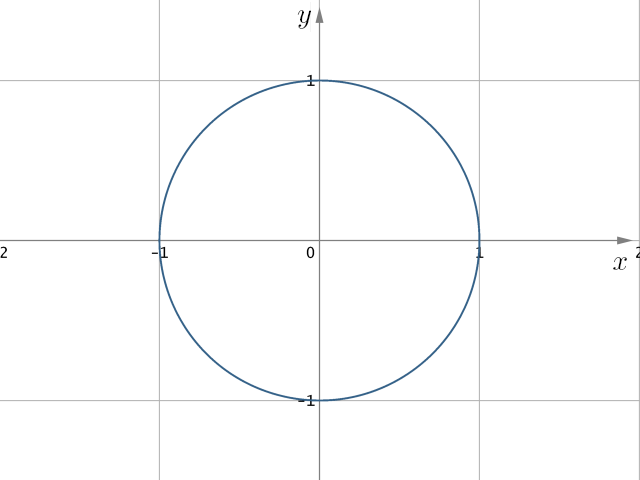
\includegraphics[scale=0.2]{img/kreis/kreis1.png}
\end{center}

Koordinatengleichung:
\[x^2 + y^2 = 1 \]

\item Kreis mit Radius $r = \sqrt 2$ und Mittelpunkt $M = (\sqrt 2 , \sqrt 2)$:

\begin{center}
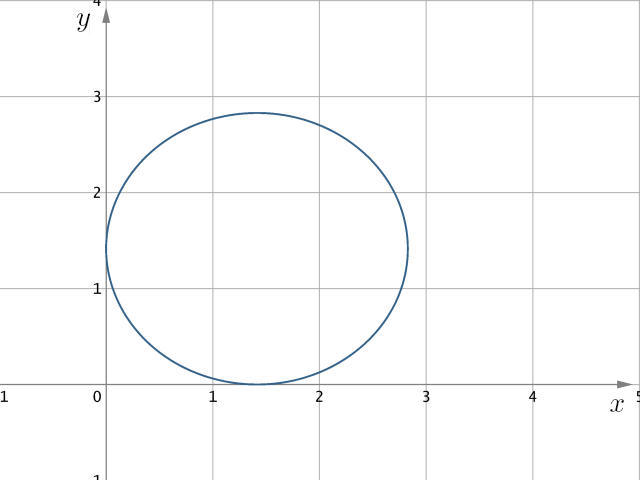
\includegraphics[scale=0.2]{img/kreis/kreis2.png}
\end{center}

Koordinatengleichung:
\[(x - \sqrt 2)^2 + (y - \sqrt 2)^2 = 2 \]


\item Oberer Halbkreis mit Radius $r = 1.5$ und Mittelpunkt $M = (4 , 3)$

\begin{center}
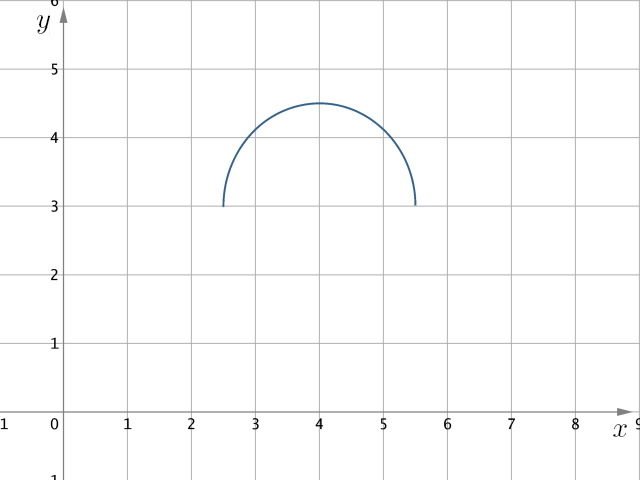
\includegraphics[scale=0.2]{img/kreis/kreis3.png}
\end{center}
Funktionsgleichung: 
\[y = 3 + \sqrt{ 2.25 - (x - 4)^2} \]

\end{enumerate}

\subsection{Aufgaben}
\begin{enumerate}
\item Stellen Sie die Kreisgleichung f"ur einen Kreis mit dem Mittelpunkt M auf, der durch den Punkt $P_1$ geht.
\begin{enumerate}
\item $M(1|3) ; P(4|3)$
\item $M(-1| 5) ; P(6|-4)$
\item $M(-2|-1) ; P(4|3)$
\end{enumerate}
\item Welches geometrische Objekt wird durch die Gleichung beschrieben? Skizzieren Sie dieses in einem Koordinatensystem
\begin{enumerate}
\item $x^2 + y^2 - 4x - 2y + 5 = 4$
\item $x^2 + y^2 + 6x + 2y + 10 = 1$
\end{enumerate}

\item * Geben Sie die Gleichung des Kreises an, der durch die Punkte $P_1(6|7), P_2(2|9) $und $P_3(-1|0)$ geht.

\end{enumerate}

